\documentclass[12pt, twoside]{article}
\usepackage[letterpaper, margin=1in, headsep=0.5in]{geometry}
\usepackage[english]{babel}
\usepackage[utf8]{inputenc}
\usepackage{amsmath}
\usepackage{amsfonts}
\usepackage{amssymb}
\usepackage{tikz}
\usetikzlibrary{quotes, angles}
\usepackage{graphicx}
%\usepackage{pgfplots}
%\pgfplotsset{width=10cm,compat=1.9}
%\usepgfplotslibrary{statistics}
%\usepackage{pgfplotstable}
%\usepackage{tkz-fct}
%\usepackage{venndiagram}

\usepackage{fancyhdr}
\pagestyle{fancy}
\fancyhf{}
\renewcommand{\headrulewidth}{0pt} % disable the underline of the header

\fancyhead[RE]{\thepage}
\fancyhead[RO]{\thepage \\ Name: \hspace{3cm}}
\fancyhead[L]{BECA / Dr. Huson / Geometry 10th Grade\\* Unit 3: Volume and angle bisectors \\ 
2 October 2019}

\begin{document}
\subsubsection*{3.1 Homework: Volume and vertical angles}
  \begin{enumerate}

  \item As shown below, two lines intersect making four angles: $\angle 1$, $\angle 2$, $\angle 3$, and $\angle 4$.
    \begin{center}
    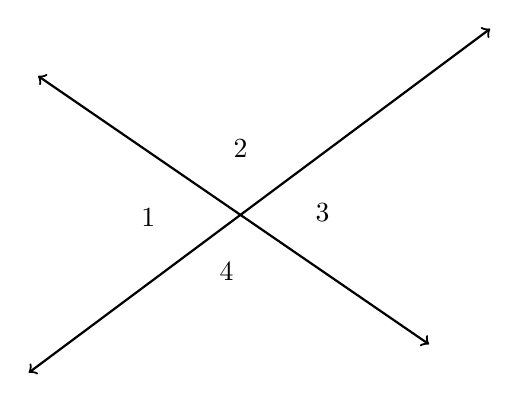
\begin{tikzpicture}[scale=0.7, rotate=20]
      \draw [<->, thick] (0,-1.5)--(10,1.5);
      \draw [<->, thick] (2,3.5)--(7,-3.5);
      \node at (3,.4){1};
      \node at (6,-.6){3};
      \node at (5,1){2};
      \node at (4,-1){4};
      %\draw [fill] (0,0) circle [radius=0.05] node[below]{$P$};
      %\draw [fill] (6,0) circle [radius=0.05] node[below]{$R$};
      %\draw [fill] (3,0) circle [radius=0.05] node[below]{$Q$};
    \end{tikzpicture}
    \end{center}
    \begin{enumerate}
    \item Given that $m\angle 1= 75^\circ$, find $m\angle 2=$ \rule{2.5cm}{0.15mm} \bigskip
    \item Find $m\angle 3=$ \rule{2.5cm}{0.15mm} \bigskip
    \item True or false, $\angle 1$ and $\angle 4$ are supplementary angles. \rule{3cm}{0.15mm}
  \end{enumerate}

  \item Given the rectangle $ABCD$ shown below, with $AB=6 \frac{1}{3}$ and $BC=2 \frac{1}{2}$. Find the area of the rectangle, expressing your result as a fraction.
\begin{flushright}
\begin{tikzpicture}[scale=1.25]
  \draw [-, thick] (0,0)--(4.5,0)--(4.5,2)--(0,2)--cycle;
  \draw [fill] (0,0) circle [radius=0.05] node[left]{$A$};
  \draw [fill] (4.5,0) circle [radius=0.05] node[right]{$B$};
  \draw [fill] (4.5,2) circle [radius=0.05] node[right]{$C$};
  \draw [fill] (0,2) circle [radius=0.05] node[left]{$D$};
  \node at (5, 1){$2 \frac{1}{2}$};
  \node at (2.25, -0.5){$6 \frac{1}{3}$};
\end{tikzpicture}
\end{flushright} \vspace{2cm}  

\item Find the volume of a box (rectanglar prism) having a length of 12 inches, a width of 6 inches, and a height of 5 inches. Show the calculation.

\newpage
  \item The Washington Monument has a square base 55 feet long on each side. It is roughly 555 feet tall. Estimate its volume using the formula for a prism. (in fact, the sides angle in slightly and the monument is narrower at the top)  \vspace{7cm}  

  \item Measure the required angles of the diagram below and answer the questions. \vspace{0.25cm}
  \begin{enumerate}
    \item  $m \angle AOB = $ \rule{2.5cm}{0.15mm} \hspace{0.5cm} $m \angle BOC = $ \rule{2.5cm}{0.15mm} \hspace{0.5cm} $m \angle DOE = $ \rule{2.5cm}{0.15mm}\bigskip
    \item Name the angle that is opposite to $\angle AOB$: \rule{4cm}{0.15mm}  \bigskip
    \item Name an angle that is supplementary to $\angle COB$: \rule{4cm}{0.15mm} \bigskip
    \item Name an angle that is complementary to $\angle DOE$: \rule{4cm}{0.15mm}
  \end{enumerate}
  \vspace{1cm}
  \begin{center}
  \begin{tikzpicture}[scale=1.3, rotate=20]
    \draw [<->, thick] (-25:5)--(0,0)--(155:5);
    \draw [<->, thick] (-5,0)--(5,0);
    \draw [->, thick] (0,0)--(0,4);
    \draw (0,0)++(0.3,0)--++(0,0.3)--+(-0.3,0);
    %\draw [fill] (-1,2.5) circle [radius=0.05] node[left ]{$B$};
    \draw [fill] (155:3) circle [radius=0.05] node[below left]{$B$};
    \draw [fill] (-4,0) circle [radius=0.05] node[below]{$A$}; 
    \draw [fill] (0,0) circle [radius=0.05] node[below left]{$O$};
    \draw [fill] (0,3) circle [radius=0.05] node[left]{$C$};
    \draw [fill] (4,0) circle [radius=0.05] node[below]{$D$};
    \draw [fill] (-25:2) circle [radius=0.05] node[below]{$E$};
  \end{tikzpicture}
  \end{center}

  \newpage

\end{enumerate}
\end{document}
